\documentclass[12pt]{article}
\usepackage{enumerate}
\usepackage{amsmath}
\usepackage{amssymb}
\usepackage{amsthm}
\usepackage{etoolbox}
\usepackage{graphicx}

\newcommand{\Name}[1]{\noindent \textbf{Name:} #1 \\}
\newcommand{\Workedwith}[1]{\noindent \textbf{Worked with:} #1 \\}
\newcommand{\Problem}[3]{\mbox{} \newline \noindent \textbf{\textbf{Problem #1: #2 [#3 Points] \\ }}}


\begin{document}

\begin{center}
  \bf
  Algorithms \\
  CMPT 307 D200 \\
  Spring 2024 \\
  \rm
  Homework 5\\
  Due:  Sunday, Mar 31 at 10:00 PM \\
\end{center}

\Name{Sara Magdalinski}
\Workedwith{N/A}

\Problem{5}{Gamesville}{20}

Many puzzles can be solved by transforming (or ``reducing'') them to network flow problems.  That's what you'll do here, like the last problem!

A different popular online gaming website, Gamesville, has a puzzle on their website called Defective Chess Boards. DCB is a puzzle that goes like this:  We're given an $n \times n$ chessboard in which some cells are missing.  The goal is to tile the board with dominoes, each of which covers exactly two adjacent cells, or determine
that no such tiling exists.  Figure~\ref{fig:dominoes} shows a defective chess board and a valid tiling.  Describe an algorithm for determining whether or not a given $n \times n$ defective chess board has a valid tiling and, if it does, to find that tiling.  Prove
that your algorithm is correct and give its running time as a function of $n$.  You should assume that the input defective chess board is given to us as an $n \times n$ matrix where each entry in the matrix indicates if the corresponding cell in the board is black, white, or missing.

\begin{figure}[h]
\begin{center}
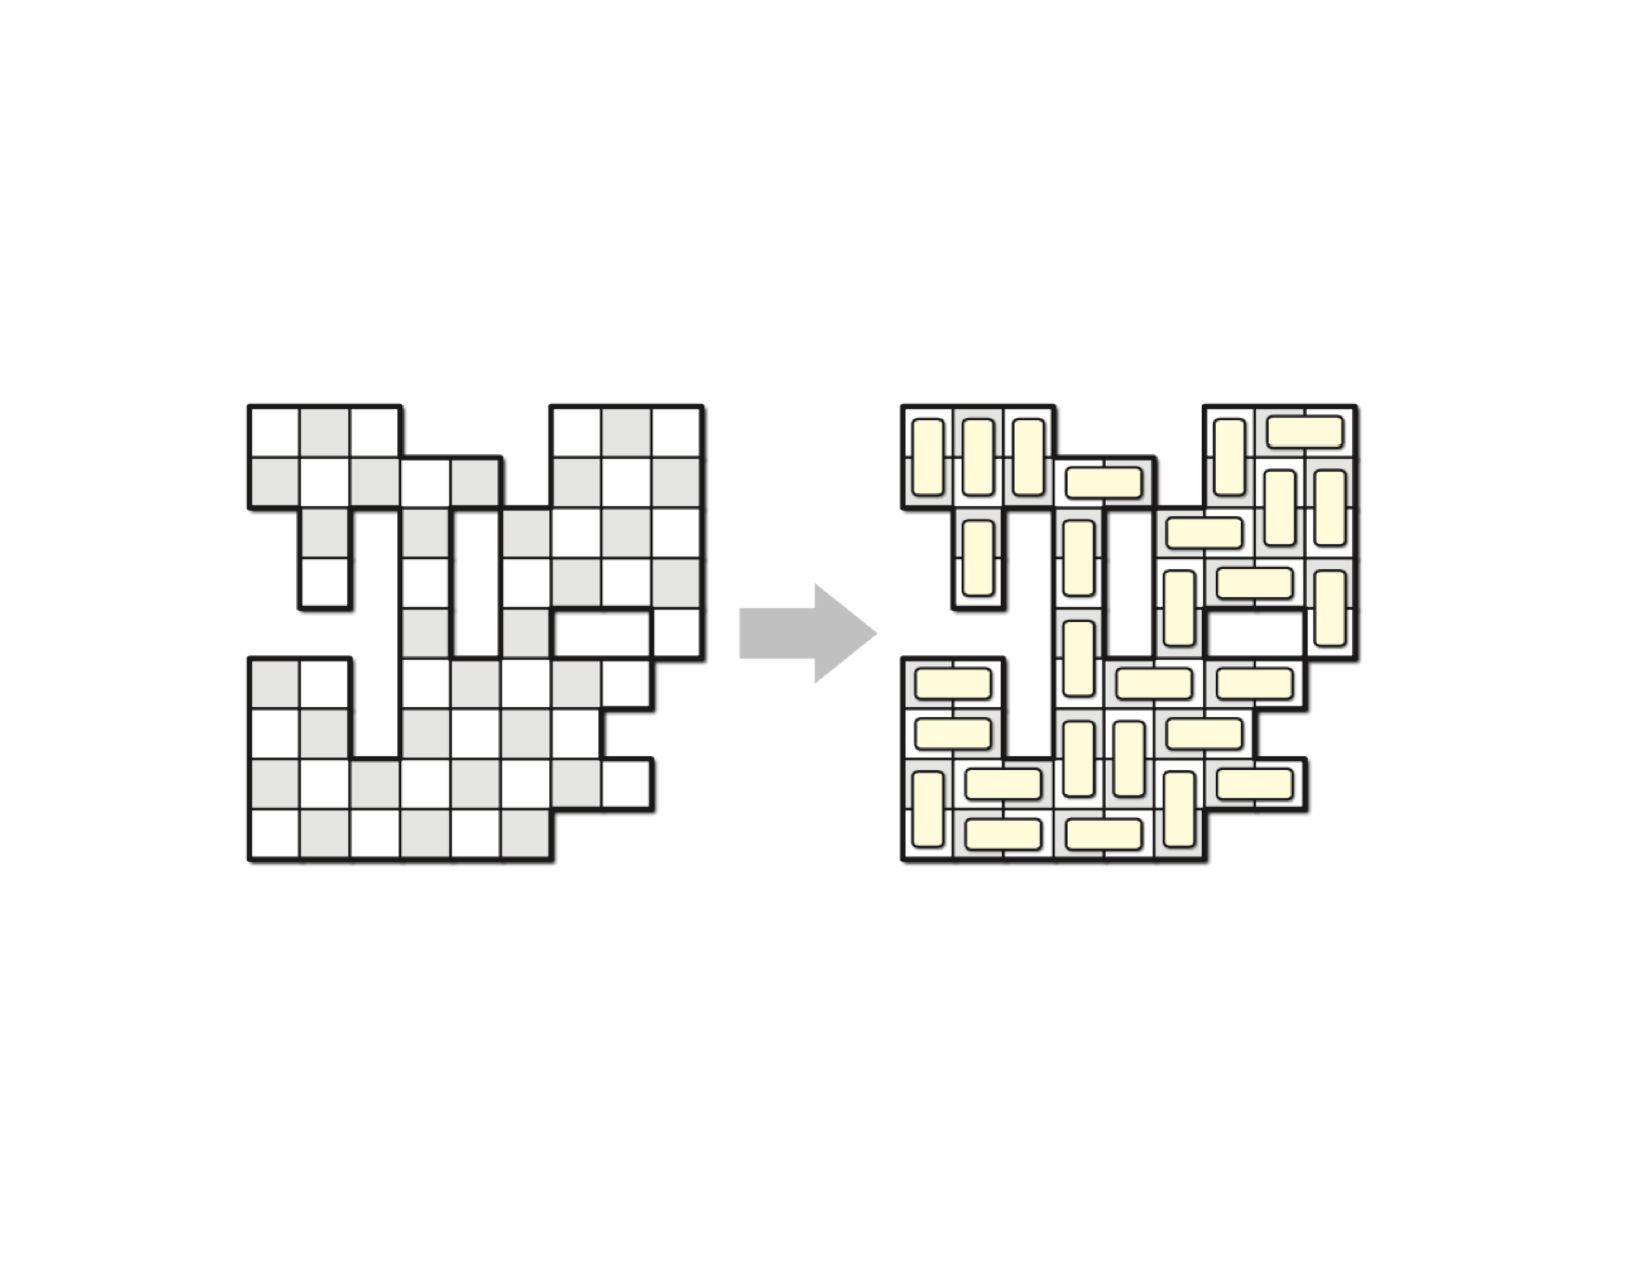
\includegraphics[width=4in]{Dominoes.pdf}
\end{center}
\caption{A defective chessboard and a tiling of that board with dominoes.}
\label{fig:dominoes}
\end{figure}

\textbf{Solution:}
Part 1: Reduction: We can reduce this problem into a network flow problem. To do this we must note that a domino must be placed on one black tile and one white tile since no two black cells are adjacent and no two white cells are adjacent. This allows us to form a bipartite graph G (V = A $\cup$ B, E) where A and B represent the two distinct vertex sets and can be used to provide a solution using a network flow algorithm. We will let the vertex set A represent the black tiles and the vertex set B represent the white tiles. In order for a solution to be found we must have the same number of white and black tiles (i.e the same number of vertices in A and B) which implies we must have an even number of tiles, if this invariant is broken we know there is no possible solution. Given this invariant we can say that A and B each have some number of vertices m where m is $\le \frac{n^2}{2}$ since we have $n^2$ tiles (including white, black and missing) and at most half are white and at most half are black. We can label the vertices in a and b from 1 to m. For simplicity when finding the valid tiling we will label them in order left to right, top to bottom skipping tiles that are the opposite color/missing. We will then add edges between adjacent tiles. We will just add directed edges from A to B (black to white) as this will cover all possible domino placements. If an adjacent tile is missing, we will not add any edge. We then need to add a start node, lets say S, that has a directed edge to every vertex in A (black tiles) and an end node, lets say N, that has a directed edge from every vertex in B (white tiles). We will set each edge to have a weight of 1. This problem has now been reduced to a network flow problem and we can solve it using the Ford-Fulkerson algorthm which will determine the maximum flow in the network. We will know a solution is possible if the maximum flow is equal to m (note we have m black and m white tiles) since each unit of flow from the source node to the end node represents 1 domino being placed on two adjacent (one black (A), one white (B)) tiles. If we have a maximum flow of m that means that every tile has been covered by a domino. To find this valid tiling, while running the Ford Fulkerson algorithm when an edge is chosen to be used between A and B we will remember the vertexes chosen in A and B by adding them as a tuple into a solution array. \\

Step 2: Proof of correctness: 
Now, we prove that the reduction is correct. This involves two steps: first we must prove that the edges we’ve selected provide a valid way to place the dominoes, then we must prove that there does not exist a solution consisting of more dominos.
First, we want to show that this solution is valid. Assume by way of contradiction that this solution is not valid. This means that either one of the vertices in A has two or more outgoing edges selected in our solution, or one of the vertices in B has two or more incoming edges selected. Well, neither of these are possible, since we only select an edge to put in our solution if the corresponding edge in the Network Flow graph has a flow of 1 through it, and there can only be one unit of flow that makes it to any vertex in A, and only one unit of flow can leave from any vertex in B! Thus, we have reached a contradiction and our assumption was correct; thus, this is a valid way to place the dominoes. Next, we will show that it is in fact the largest possible number of dominoes. Assume by way of contradiction that there is a larger possible number of dominoes. We can now construct a flow through our graph using this new larger number of dominoes (i.e edges from A to B) that exceeds the previous max flow we computed. However, that’s a contradiction, because Ford-Fulkerson is a correct algorithm! Thus, this is the maximum number of dominoes.

Step 3: Time Efficiency: We will split this into three parts. Constructing our graph, evaluating the problem using the Ford Fulkerson algorithm, and transforming it back into the solution we need.\\

Constructing the graph: We will have to iterate over the entire original n x n board which consists of $n^2$ tiles (missing, white, black) in order to create our graph. For each tile, if it is black we will assign it a number between 1 and m in the way described when performing the reduction. We will do the same for white tiles. This step will take O($n^2$) time.  We will then iterate over the set of black tiles (at most $\frac{n^2}{2}$) and for each adjacent tile (at most four so O(1)) if it is missing we will do nothing and if it is white we will add an edge from the black tile to the white tile (A$\rightarrow$B). This step will take O($\frac{n^2}{2}$) time in the worst case which can be written as O($n^2$). We will then add a vertex S which is our start/source and add directed edges from S to each vertex in A which is at most $\frac{n^2}{2}$ edges. We will do the same to connect each vertex in B to N (end/sink) which is another at most $\frac{n^2}{2}$ edges. This step will take at most O($n^2$) time as well. So, in total for constructing the graph we have a time efficency of O($n^2$ + $n^2$ + $n^2$) which can be simply written as O($n^2$).\\

Running the algorithm: The Ford-Fulkerson algorithm takes O(E * F) where E is the number of edges and F is the maximum flow. This algorithm is optimal for this problem as the maximum flow is less than $n^2$. The number of edges in the graph is at most $\frac{n^2}{2}$ from S to all the vertexes in A, plus at most 4$\frac{n^2}{2}$ edges from A to B (since a tile is adjacent to at most 4 other tiles), plus at most $\frac{n^2}{2}$ edges from B to N. The maximum flow is m where m is $\le \frac{n^2}{2}$. This shows that the time efficiency of the Ford-Fulkerson algorithm in this case is O((6$\frac{n^2}{2}$) * $\frac{n^2}{2}$) = O(6$\frac{n^4}{4}$) = O($n^4$). To find the actual tiles on which we will place dominoes we will store the selected edges in the algorithm into another data structure, this will not impact the time efficiency as it is simply an O(1) step that we are adding to the existing algorithm (assuming this is an adjustment we can make to the Ford-Fulkerson algorithm as the actual process of this algorithm was not explained in class - solely the time efficiency was noted to be of importance). To loop through the array and rebuild the graph it would take at most O($n^2$) time which would still not impact the running time.\\

Providing the solution: We are simply returning if a valid solution exists and the array we created containing the placement of the dominoes if this solution exists which is O(1). We have a valid solution when the Ford-Fulkerson algorithm returns a max flow of m where m is the number of black tiles (we also have m white tiles).\\

Overall time efficiency: O($n^2$ + $n^4$ + 1) = \emph{O($n^4$)}.





 




\end{document}
